\documentclass[14pt]{extarticle} %Класс позволяет использовать базовые шрифты бОльших размеров
\usepackage{imit_vkr}

%=============================
%Персональная настройка макета
%Здесь могут располагаться дополнительные команды для персональной тонкой настройки
%=============================

%=============================
%Конец Персональная настройка макета
%=============================

%Подключение литературы
\addbibresource{literature.bib}
\begin{document}
	
%%%--------Титульная страница
%==Титульная страница
\thispagestyle{empty}
\begin{center}
Министерство науки и высшего образования Российской Федерации\\
Федеральное государственное бюджетное образовательное\\
учреждение высшего образования\\
<<Иркутский государственный университет>>\\
(ФГБОУ ВО <<ИГУ>>)\\
Институт математики и информационных технологий\\
Кафедра алгебраических и информационных систем\\
\end{center}

\vspace{2.7cm}

\begin{center}
{\bf 
КУРСОВАЯ РАБОТА\\[1mm]
по предмету\\[1mm]
<<Проектирование информационных систем>>
}  

\vspace{0.9cm}

{
РАЗРАБОТКА ВЕБ-ПРИЛОЖЕНИЯ\\[1mm]
ДЛЯ ВЫБОРА ТЕМЫ КУРСОВОЙ РАБОТЫ
}
\end{center}

\vspace{2.3cm}

{
\noindent\hbox to 0.48\textwidth {%
	\mbox{ } \hfil} %
	\begin{tabular}[t]{l}
		Студент 3 курса очного отделения\\
		Группа 02361--ДБ\\
		Петров Иван Алексеевич		
	\end{tabular}		
}

\vspace{1.3cm}

{
\noindent\hbox to 0.48\textwidth {%	
	\mbox{ } \hfil} %
	\begin{tabular}[t]{l}
		Руководитель:\\ к.ф.-м.н., доцент Рябец Л.В.		
	\end{tabular}		
}


\vfill 
\noindent
\begin{minipage}{\textwidth}
\centering	 Иркутск 2024
\end{minipage}
%%%----------------------Содержание дипломной работы%%%
\renewcommand{\baselinestretch}{1.5}
\normalsize
%-------------
%Содержание
%-------------
\renewcommand{\contentsname}{СОДЕРЖАНИЕ}
\noindent\tableofcontents

%-------------
%Основная часть
%-------------
\mynonumbersection{ВВЕДЕНИЕ}

Современные информационные технологии играют важную роль в организации образовательного процесса. Развитие веб-приложений открывает новые возможности для автоматизации различных аспектов учебной деятельности, включая выбор тем для курсовых работ. Традиционно процесс выбора темы курсовой работы осуществлялся на основании консультаций с преподавателями и поиска информации по различным источникам. Однако такой подход зачастую оказывается трудоемким и неэффективным, особенно в условиях увеличения объемов информации и количества студентов.
Веб-приложение для выбора темы курсовой работы направлено на оптимизацию этого процесса. Основная цель разработки заключается в создании удобного инструмента, который позволит студентам быстрее и легче находить подходящие темы на основе их интересов, академической успеваемости и рекомендаций преподавателей. 
\textbf{Целью} данного проекта является разработка рабочего, функционального веб-приложения для выбора тем курсовых работ.


\textbf{Задачи}:
\begin{enumerate}
    \item Разработать компактный список тем курсовых работ;
    \item Реализовать возможность предложения своей темы;
    \item Реализовать комментирование тем курсовых работ;
    \item Реализовать регистрацию и авторизацию пользователей;
    \item Реализовать функцию обмена сообщениями.
\end{enumerate}
\newpage

Выбор Spring Boot для backend и React для frontend обусловлен целью создания удобного и отзывчивого приложения для выбора темы курсовой работы. Spring Boot обеспечивает высокую надежность и масштабируемость, что особенно важно для стабильной работы системы. Кроме того, он значительно упрощает процесс разработки и развертывания благодаря встроенным инструментам и автоматической настройке. React, в свою очередь, позволяет создавать динамичный и интерактивный пользовательский интерфейс за счет использования компонентов и широких возможностей для управления состоянием.

Для работы с данными выбрана база данных MySQL, так как она предлагает эффективные и надежные инструменты для хранения информаци. Эти технологии обеспечивают надежный фундамент для разработки приложения, которое сочетает в себе высокую скорость работы, интерактивность и удобство для пользователей.


%=======================

\mysection{Описание предметной области}
\mysubsection{Анализ предметной области}

Первый аспект, требующий внимания, — это неопределенность интересов студентов при выборе темы курсовой работы. Широкий спектр доступных тем может сбивать с толку, особенно для тех, кто только начинает свой путь в академической среде. Этот момент подчеркивает необходимость разработки эффективных инструментов \textit{поддержки и рекомендаций}, которые помогут студентам быстрее ориентироваться в возможных вариантах и выбирать наиболее подходящие темы, учитывая их академические интересы и карьерные цели.

Второй аспект --- это потребность в автоматизации процессов, связанных с выбором тем курсовых работ. Информационная система должна предоставлять пользователям удобные инструменты для коммуникации с преподавателем и \textit{выбором темы}.

Кроме того, важно учитывать интересы аудитории, заинтересованной в моей платформе. Это \textbf{студенты} и \textbf{преподаватели}, стремящиеся оптимизировать процесс выбора тем для курсовых работ. \textbf{Студенты} хотят получить удобный инструмент для поиска тем, который позволит им быстро находить подходящие варианты, учитывая их академические интересы и навыки. Они также заинтересованы в прозрачности процесса, чтобы видеть актуальные темы и отслеживать статус своей заявки.

\textbf{Преподаватели}, в свою очередь, стремятся упростить управление темами, облегчить взаимодействие со студентами и снизить административную нагрузку. Им важно, чтобы платформа предоставляла гибкие инструменты для создания и редактирования тем, распределения студентов по темам и контроля за выполнением учебных требований.

Аналогов этой системы, которые были бы ориентированы на выбор темы курсовой работы, не известно, поскольку данная тема является узконаправленной. Как правило, подобные приложения разрабатываются не для общего пользования, а для конкретных учебных заведений, что ограничивает их доступность и функциональность. Это создает уникальную нишу для моего проекта, позволяя сосредоточиться на потребностях студентов и преподавателей, обеспечивая более гибкий и удобный инструмент для выбора тем курсовых работ.


\mysubsection{Требования к разрабатываемому приложению}

Разработка веб-приложения для темы курсовой работы должна соответствовать определенным требованиям, чтобы обеспечить его функциональность, простоту использования и надежность. Вот основные требования к разрабатываемому приложению:

\begin{itemize}
    \item \textbf{Возможность оставлять комментарии}: 
Приложение предоставляет возможность преподавателям комментировать темы, предложенные студентами. Это создает интерактивную атмосферу, в которой студенты могут получать обратную связь и рекомендации от преподавателей, что способствует более осознанному выбору тем курсовых работ. Такой функционал помогает пользователям принимать более информированные решения и повышает качество взаимодействия между студентами и преподавателями.
    \item \textbf{Обработка ошибок и исключений}: приложение обеспечивает надежную обработку ошибок и исключений, что гарантирует стабильную работу сервиса и минимизирует возможные проблемы во время использования.
    \item \textbf{Удобная работа с темами для преподавателей}: для преподавателей предусмотрены инструменты для управления содержимым, что обеспечивает эффективное управление списком тем.
    \item \textbf{Возможность добавления своей темы}: Студенты могут легко отправлять свои темы на рассмотрение преподавателям. Если тема одобряется и соответствует требованиям, она утверждается. Этот процесс обеспечивает прозрачность и дает студентам возможность получить обратную связь, что повышает вероятность выбора актуальной и интересной темы для курсовой работы.
\end{itemize}


Для разработки приложения было важно рассмотреть проект с перспективы как студентов, так и преподавателей. Выделим несколько способов, которыми пользователи могут взаимодействовать с моим приложением. Это позволяет создать более полное и эффективное решение, отвечающее потребностям обеих сторон:

\begin{longtable}{|p{3cm}|p{14cm}|}
\hline
ID & 1 \\ \hline
Заголовок & Выбор темы курсовой работы\\ \hline
Описание & Студент находит и выбирает понравившуюся пластинку при пом списка тем курсовых работ\\ \hline
Основной актёр & Зарегистрированный студент\\ \hline
Предусловия & Студент авторизован в системе \\ \hline
Постусловия & Студент выбрал тему\\ \hline
Основной сценарий & 
1. Студент нажимает кнопку «Свободные темы»

2. Система отображает список свободных тем курсовых работ

3. Студент выбирает понравившуюся тему

4. Система выводит подробную информацию о теме курсовой работы

7. Студент нажимает кнопки "выбрать" \, и "подтвердить"

8. Система фиксирует тему, предложенную студентом, а также удаляет ее из списка достпуных тем.

9. Студент нажимает кнопку "Выбранная тема"

10. Система выводит информацию о выбранной теме пользователя.\\ \hline

Приоритет & Высокий
\\ \hline	
\end{longtable}

\begin{longtable}{|p{3cm}|p{14cm}|}
\hline
ID & 2 \\ \hline
Заголовок & Предложение своей темы\\ \hline
Описание & Студент заполняет информацию о предлагаемой теме и консультируется с преподавателем\\ \hline
Основной актёр & Зарегистрированный студент\\ \hline
Предусловия & Студент авторизован в системе \\ \hline
Постусловия & Студент выбрал тему, предложенную им самостоятельно \\ \hline
Основной сценарий & 
1. Студент нажимает кнопку «Свободные темы»

2. Система отображает список свободных тем курсовых работ

3. Студент не находит подходяшую тему

4. Студент нажимает кнопку "Предложить свою тему"

5. Система выводит форму для заполнения

6. Студент вводит информацию о предлагаемой теме

7. Студент нажимает кнопку "предложить"

8. Студент ждёт комментария или одобрения темы от преподователя

9. Студент корректирует тему

10. Преподователь одобряет тему

11. Система фиксирует тему, предложенную студентом
\\ \hline	
Приоритет & Высокий
\\ \hline	
\end{longtable}



%==============
\mysection{Обзор технологий разработки}

Для создания веб-приложения были выбраны современные технологии, которые обеспечивают высокую производительность, надежность и удобство использования. Эти технологии позволят разработать приложение, отвечающее всем потребностям пользователей. 

\mysubsection{Spring Boot}


Spring Boot был выбран в качестве основного фреймворка для разработки серверной части приложения из-за своей надежности и отличных возможностей масштабирования ~\cite{SpringBoot}. Этот фреймворк на Java предоставляет широкий спектр встроенных инструментов и автоматизированных настроек, что значительно облегчает как процесс разработки, так и его последующее развертывание. Благодаря Spring Boot можно оперативно настраивать и запускать серверную часть, а также эффективно интегрировать различные компоненты приложения.

Одной из наиболее заметных черт Spring Boot является его легковесная архитектура, которая способствует высокой производительности. Он поддерживает множество баз данных и технологий интеграции, что делает его идеальным выбором для разработки сложных веб-приложений ~\cite{Spring.NET}. Кроме того, обширная экосистема и активное сообщество разработчиков обеспечивают наличие качественной документации и примеров, что делает процесс разработки более доступным и менее трудоемким.

\mysubsection{React}

React был выбран для разработки интерактивного и отзывчивого пользовательского интерфейса благодаря своей популярности и широким возможностям. Эта библиотека на JavaScript позволяет создавать компоненты, которые легко повторно использовать и обновлять. React обеспечивает высокую производительность благодаря виртуальному DOM, который минимизирует количество операций с реальным DOM, что значительно ускоряет обновление интерфейса~\cite{ReactDevBlog}.

Кроме того, React предлагает обширный набор инструментов и библиотек, таких как React Router для управления маршрутизацией и Redux для управления состоянием приложения. Эти инструменты позволяют разрабатывать сложные и динамичные пользовательские интерфейсы, которые легко поддерживать и расширять. Используя React, пользователи могут наслаждаться плавным и быстрым откликом интерфейса, что делает взаимодействие с приложением более удобным и эффективным.

\mysubsection{MySQL}

MySQL была выбрана в качестве системы управления базами данных из-за своей надежности, высокой производительности и широкого распространения. Она обеспечивает эффективное хранение и обработку данных, которые необходимы для работы приложения, включая информацию о пользователях, каталог виниловых пластинок и заказы. MySQL отличается масштабируемостью и гибкостью, что позволяет ей легко справляться с увеличением объема данных и ростом числа пользователей.

Эта система управления базами данных предлагает мощные инструменты для администрирования и возможности написания сложных SQL-запросов. Надежность и стабильность MySQL хорошо зарекомендовали себя в различных отраслях, и она активно используется для создания высоконагруженных приложений. Кроме того, MySQL поддерживает разнообразные типы данных и индексацию, что позволяет эффективно организовывать данные и быстро их извлекать, что критически важно для работы приложения.

\mysubsection{Hibernate}

Для работы с объектно-реляционным отображением (ORM) был выбран Hibernate, который значительно упрощает взаимодействие с базой данных, позволяя разработчикам работать с данными через объекты Java. Этот инструмент берет на себя автоматическое выполнение SQL-запросов и преобразование данных между объектами и таблицами базы данных, что делает код более простым и удобочитаемым.

Hibernate легко интегрируется с Spring Boot, что упрощает его настройку и использование в проекте. Он также предлагает такие возможности, как кэширование и ленивую загрузку данных, что способствует повышению производительности приложения и уменьшению числа обращений к базе данных. Применение Hibernate позволяет разработчикам сосредоточиться на бизнес-логике приложения, избавляя их от необходимости углубляться в детали работы с базой данных.

%==========================
\mysection{Описании реализации приложения}
 
\mysubsection{Хранимые сущности и проектирование структуры классов}

Чтобы лучше понять архитектуру системы, на рис. \ref{model} представлена диаграмма классов. Она иллюстрирует организацию кода и взаимодействие между различными компонентами системы, позволяя наглядно увидеть, как они связаны друг с другом.

\begin{figure}[h]
\centering
\fbox{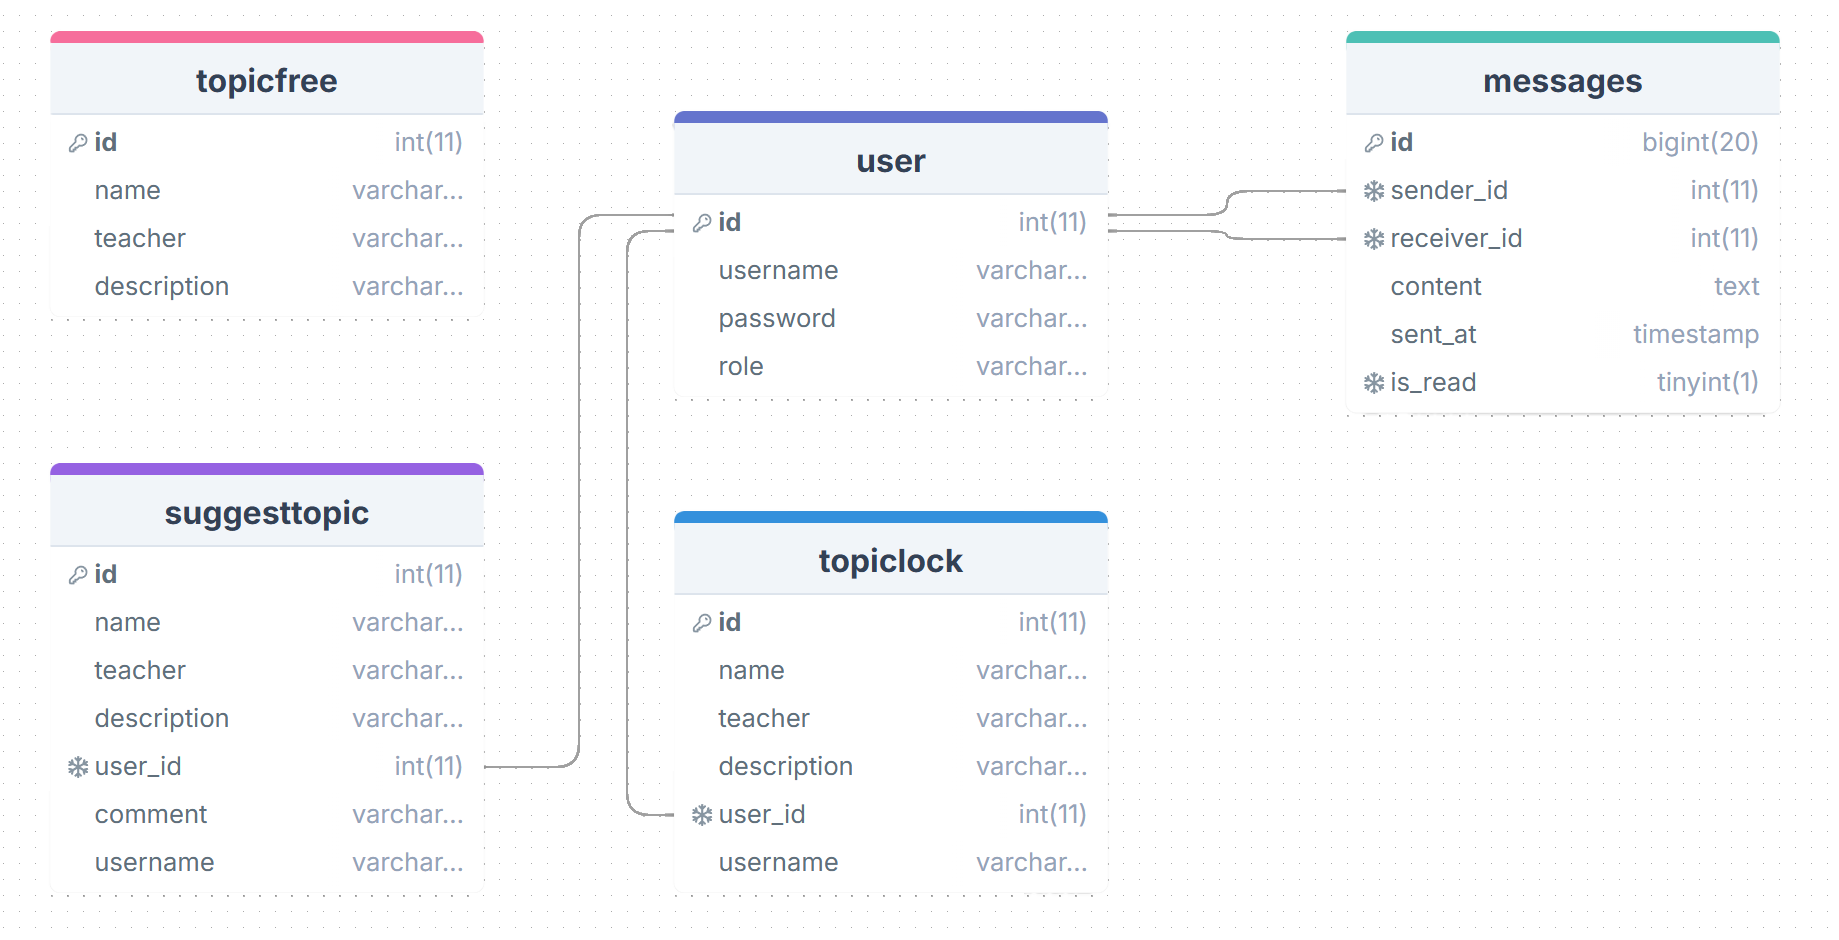
\includegraphics[scale=0.35]{cap/diagram.png}}
\caption{Диаграмма классов}
\label{model}
\end{figure}

\begin{itemize}
    \item \textbf{user}: Хранит информацию о пользователях.
    \begin{itemize}
        \item \textit{id}: Уникальный идентификатор;
        \item \textit{username}: Имя пользователя;
        \item \textit{password}: Пароль;
        \item \textit{role}: Роль пользователя.
    \end{itemize}
    \item \textbf{topicfree}: Хранит информацию о свободных темах.
    \begin{itemize}
        \item \textit{id}: Уникальный идентификатор;
        \item \textit{name}: Тема курсовой работы;
        \item \textit{teacher}: Научный руководитель;
        \item \textit{description}: Описание темы курсовой работы.
    \end{itemize}
    \item \textbf{suggesttopic}: Хранит информацию о темах предложенных студентами.
    \begin{itemize}
        \item \textit{id}: Уникальный идентификатор;
        \item \textit{name}: Тема курсовой работы;
        \item \textit{teacher}: Научный руководитель;
        \item \textit{description}: Описание темы курсовой работы;
        \item \textit{user\_id}: Уникальный идентификатор студента;
        \item \textit{comment}: Комментарий преподавателя;
        \item \textit{username}: ФИО студента.
    \end{itemize}
    \item \textbf{topiclock}: Хранит информацию о занятых темах.
    \begin{itemize}
        \item \textit{id}: Уникальный идентификатор;
        \item \textit{name}: Описание темы курсовой работы;
        \item \textit{teacher}: Научный руководитель;
        \item \textit{description}: Описание темы курсовой работы;
        \item \textit{user\_id}: Уникальный идентификатор студента;
        \item \textit{username}: ФИО студента.
    \end{itemize}
    \item \textbf{messages}: Хранит сообщения между студентами и преподавателями.
    \begin{itemize}
        \item \textit{id}: Уникальный идентификатор;
        \item \textit{sender\_id}: Идентефикатор отправителя;
        \item \textit{receiver\_id}: Идентификатор получателя;
        \item \textit{content}: Сообщение;
        \item \textit{sent\_at}: Время отправки сообщения;
        \item \textit{is\_read}: Статус получения сообщения.
    \end{itemize}
\end{itemize}   

Проект состоит из нескольких основных структур:
\begin{enumerate}[label=\arabic*)]
    \item сущности;
    \item контроллеры;
    \item репозитории;
    \item сервисы;
    \item другие классы (классы исключений, вспомогательные классы).
\end{enumerate}

ORM (Object-Relational Mapping) — это концепция, которая позволяет сопоставлять объекты из объектно-ориентированного программирования (ООП) с таблицами реляционных баз данных. В рамках этой концепции используются сущности — простые Java-объекты (POJO), которые представляют собой классы, сохраняемые с помощью библиотеки Hibernate и соответствующие определенным таблицам базы данных.

Список используемых сущностей:
\begin{enumerate}
    \item User;
    \item TopicFree;
    \item SuggestedTopic;
    \item TopicLock.
\end{enumerate}

User используется для хранения информации о пользователях системы. Эта сущность содержит основные данные пользователя, такие как имя пользователя, пароль, баланс кошелька и роль, а также имеет связь с комментариями, которые пользователь может оставлять (см. листинг \ref{lst:user}).

\begin{lstlisting}[language=Java, caption={Сущность User}, label={lst:user}]
@Entity
@Table(name = "user",
       uniqueConstraints = {@UniqueConstraint(columnNames = "username")})
@Getter
@Setter
public class User {
  @Id
  @GeneratedValue(strategy = GenerationType.IDENTITY)
  private Integer id;

  @NotBlank
  @Size(max = 100)
  private String username;

  @NotBlank
  @Size(max = 120)
  private String password;
  
  @Column(name = "role")
  private String role;

  public User() {}

  public User(String username, String password) {
    this.username = username;
    this.password = password;}
  
    public Collection<? extends GrantedAuthority> getAuthorities() {
        return AuthorityUtils.createAuthorityList(this.role.toString());}}
\end{lstlisting}

TopicFree используется для хранения информации о свободных темах курсовых работ (см. листинг \ref{lst:topicfree}).

\begin{lstlisting}[language=Java, caption={Сущность TopicFree}, label={lst:topicfree}]
@Entity
@Getter
@Setter
@NoArgsConstructor
@Table(name = "topicfree")
public class TopicFree {

    @Id
    @GeneratedValue(strategy = GenerationType.IDENTITY)
    private Integer id;

    @Column(name = "name", nullable = false)
    private String name;

    private String teacher;
    private String description;}
\end{lstlisting}

SuggestedTopic используется для хранения предложенных студентами тем курсовых работ, находящихся на рассмотрении.  (см. листинг \ref{lst:suggesttopic}).

\begin{lstlisting}[language=Java, caption={Сущность SuggestTopic}, label={lst:suggesttopic}]
@Entity
@Getter
@Setter
@NoArgsConstructor
@Table(name = "suggesttopic")
public class SuggestTopic {
    @Id
    @GeneratedValue(strategy = GenerationType.IDENTITY)
    private Integer id;

    @Column(name = "name", nullable = false)
    private String name;
    private String teacher;
    private String description;

    @Column(name = "user_id", nullable = false)
    private Integer userId;

    @Column(columnDefinition = "varchar(1000) default 'Нет комментария.'")
    private String comment;

    private String username;
}
\end{lstlisting}

TopicLock используется для хранения информации о занятых темах (см. листинг \ref{lst:topiclock}).

\begin{lstlisting}[language=Java, caption={Сущность TopicLock}, label={lst:topiclock}]
@Entity
@Getter
@Setter
@Table(name = "topiclock")
public class TopicLock {
    @Id
    @GeneratedValue(strategy = GenerationType.IDENTITY)
    @Column(name = "id")
    private Integer id;

    @Column(name = "name", length = 200, nullable = false)
    private String name;

    @Column(name = "teacher", nullable = false)
    private String teacher;

    @Column(name = "description", length = 2000)
    private String description;

    @Column(name = "user_id", nullable = false)
    private Integer userId;
    private String username;}
\end{lstlisting}


\mysubsection{Разработка серверной части веб-приложения}

\begin{figure}[h]
\centering
\fbox{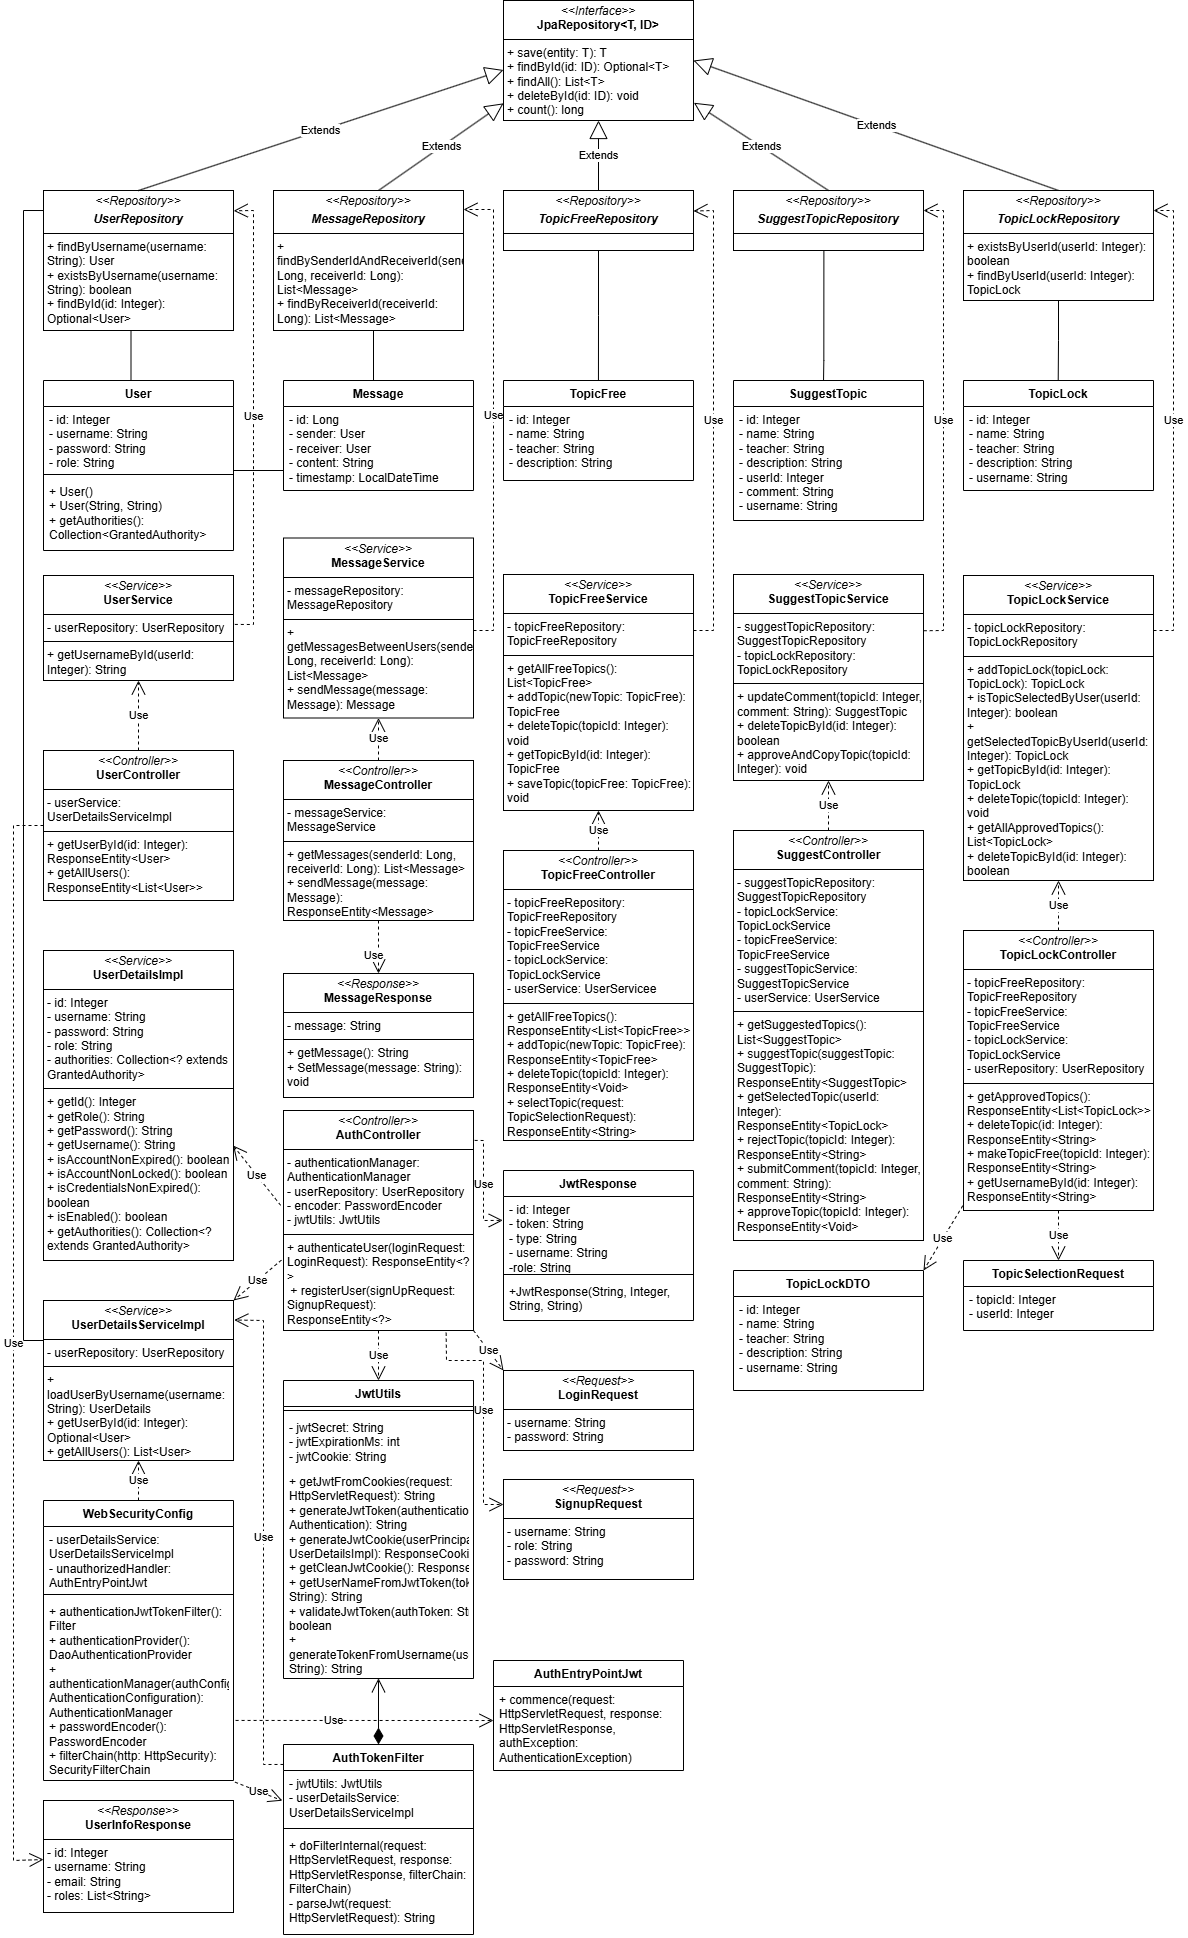
\includegraphics[scale=0.25]{cap/back.drawio.png}}
\caption{Диаграмма классов серверной части}
\label{model}
\end{figure}

Разработка серверной части веб-приложения для проекта была выполнена с использованием Spring Boot. В эту разработку входило создание контроллеров и репозиториев для управления авторизацией пользователей, работы с темами курсовых работ (создание, редактирование, удаление),  работой с комментариями, а также других функциональных возможностей.

\begin{enumerate}[label=\arabic*)]

\item В прил. \ref{topicFreeController} приведены разработанные контроллеры для управления свободными темами. Контроллеры обрабатывают запросы на создание, редактирование, удаление тем. Процесс аутентификации и авторизации включает обработку запросов на вход и выход, управление сессиями пользователей, хеширование паролей и использование JWT-токенов для обеспечения безопасности.

\item В прил. \ref{suggestTopicController} приведены разработанные контроллеры для добавления тем студентами. Контроллеры обрабатывают запросы на добавление, редактирование и удаление тем курсовых работ. 

\item В прил. \ref{topicLockController} приведены разработанные контроллеры для управления занятыми темами курсовых раб. Контроллеры обрабатывают запросы на добавление, получение, обновление и перемещение данных.

\end{enumerate}


\mysubsection{Разработка клиентской части веб-приложения}

Разработка клиентской части веб-приложения была выполнена с использованием библиотеки React. Основной задачей было создать интуитивно понятный и отзывчивый интерфейс для пользователей, который обеспечивал бы доступ ко всем функциональным возможностям приложения.



Для наглядной демонстрации внутренней работы моего проекта можно рассмотреть страницу со списком свободных тем курсовых работ. В завимости от роли и аутентификации пользователя страница показывать разное содрежимое.



ApprovedTopicsList.jsx отображает список занятых тем курсовых работ. Преподаватель может удалить тему, а ткак же перенести ее в свободные темы, дял студента эта страница не доступна (см. приложение \ref{approvedTopicsList}).

SuggestTopic.jsx отображает утвержденную для студента тему или предложенную им тему, так же содержит форму для предложения темы. Для  (см. приложение \ref{suggestTopic}).

AdminSuggestedTopics.jsx позволяет преподователям комментировать и одобрять темы студентов.

TopicFreeList.jsx отображает список тем курсовых работ. Студени может посмотреть подробную информацию о теме курсовой работе и выбрать ее. Преподователь можеть удалять и добавлять новые темы (см. листинг \ref{lst:topicFreeList}). 

\begin{lstlisting}[language=html, caption={TopicFreeList.jsx}, label={lst:topicFreeList}]
  ...
  return (
        <div className="container-md mt-3">
            <h3>Темы на согласование</h3>
            <table className="table table-bordered mt-2">
                <thead>
                    <tr>
                        <th>Имя студента</th>
                        <th>Название темы</th>
                        <th>Научный руководитель</th>
                        <th>Комментарий</th>
                        <th>Действия</th>
                    </tr>
                </thead>
                <tbody>
                    {suggestedTopics.map((topic) => (
                        <tr key={topic.id}>
                            <td>{topic.username}</td> {/* Имя студента */}
                            <td>{topic.name}</td>
                            <td>{topic.teacher}</td>
                            <td>{topic.comment || 'Нет комментария'}</td>
                            <td>
                                <button onClick={() => toggleDescription(topic.id)} className="btn btn-info">
                                    {selectedTopicId === topic.id ? "Скрыть описание" : "Подробнее"}
                                </button>
                                <button onClick={() => toggleComment(topic.id)} className="btn btn-warning ms-2">
                                    {commentTopicId === topic.id ? "Отмена" : "Комментировать"}
                                </button>
                                <button onClick={() => handleApprove(topic.id)} className="btn btn-success ms-2">
                                    Одобрить
                                </button>
                            </td>
                        </tr>
                    ))}
                </tbody>
            </table>
            {commentTopicId && (
                <div className="mt-3">
                    <textarea
                        className="form-control"
                        rows="3"
                        value={comment}
                        onChange={handleCommentChange}
                        placeholder="Введите комментарий"
                    />
                    <button
                        onClick={() => handleSubmitComment(commentTopicId)}
                        className="btn btn-primary mt-2"
                    >
                        Отправить комментарий
                    </button>
                </div>
            )}
            {suggestedTopics.map((topic) => (
                selectedTopicId === topic.id && (
                    <div className="alert alert-info mt-3" key={topic.id}>
                        <strong>Описание:</strong> {topic.description}
                    </div>
                )
            ))}
        </div>
            ...
\end{lstlisting}

\mysubsection{Реализованная функциональность}

Для наглядной демонстрации работы приложения приведены изображения и комментарии, иллюстрирующие функциональные возможности и пользовательский интерфейс.

Первая страница которую нам стоит рассмотреть --- страница регистрации пользователя. Конечно же можно посмотреть все основные вкладки можно и за не зарегестрированного пользователя, но основной функционал открывается только авторизированным пользователям. 

\begin{figure}[h]
	\centering	\fbox{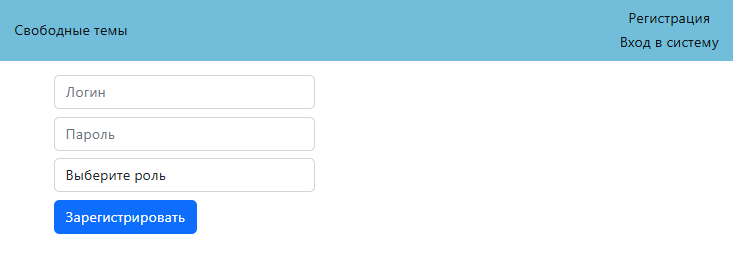
\includegraphics[width=0.8\textwidth]{cap1/registration.png}}
	\caption{Страница регистрации}
	\label{ris1}
\end{figure}
\newpage
Войдём в систему как администратор чтобы увидеть скрытые от обычных пользователей компоненты. 

\begin{figure}[h]
	\centering	\fbox{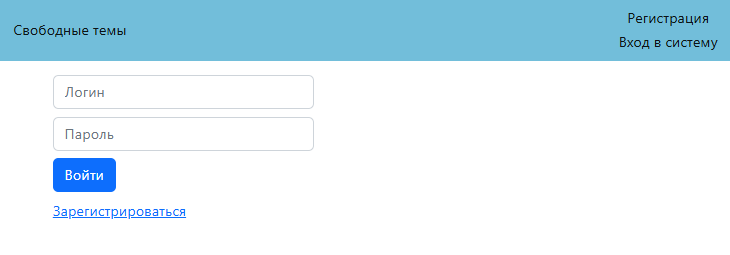
\includegraphics[width=0.8\textwidth]{cap1/authorization.png}}
	\caption{Страница авторизации}
	\label{ris1}
\end{figure}
Студенты могут только посмотреть список свободных тем, прочитать их описание и предложить свою тему, а администратор может как добавить новую тему, так и удалить старую.

\begin{figure}[h]
	\centering	\fbox{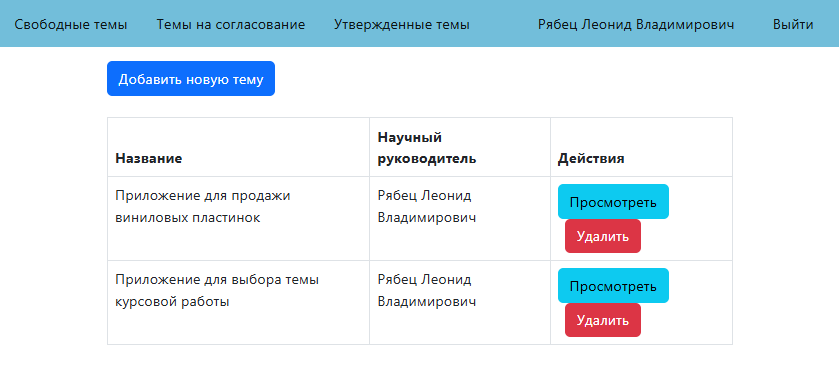
\includegraphics[width=0.8\textwidth]{cap1/listfree.png}}
	\caption{Список свободных тем}
	\label{ris1}
\end{figure}
\newpage
Темы на согласование --- это одна из самых главных страниц всего моего проекта. Здесь студенты могут проявить себя и предложить свою тему. Преподаватель может ее добавить.

\begin{figure}[h]
	\centering	\fbox{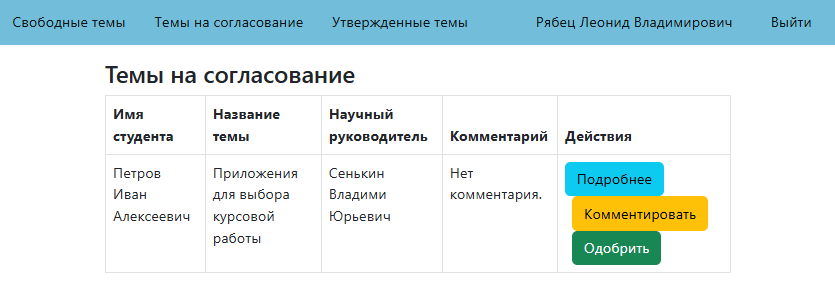
\includegraphics[width=0.8\textwidth]{cap1/sog1.png}}
	\caption{Список тем на согласование}
	\label{ris1}
\end{figure}

Для администраторов была создан удобный список с занятыми темами.
\begin{figure}[h]
	\centering	\fbox{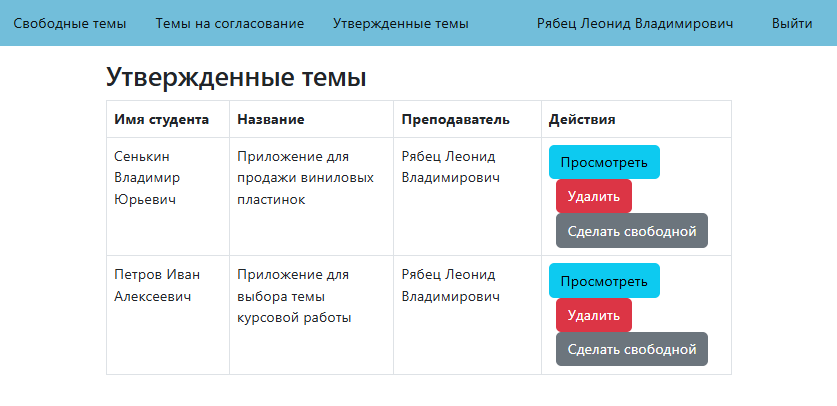
\includegraphics[width=0.8\textwidth]{cap1/utv.png}}
	\caption{Утвержденные темы}
	\label{ris1}
\end{figure}
\newpage

Для преподавателей реализована форма добавления новых тем курсовых работ, которая открывается при нажатии на кнопку "добавить новую тему".

\begin{figure}[h]
	\centering	\fbox{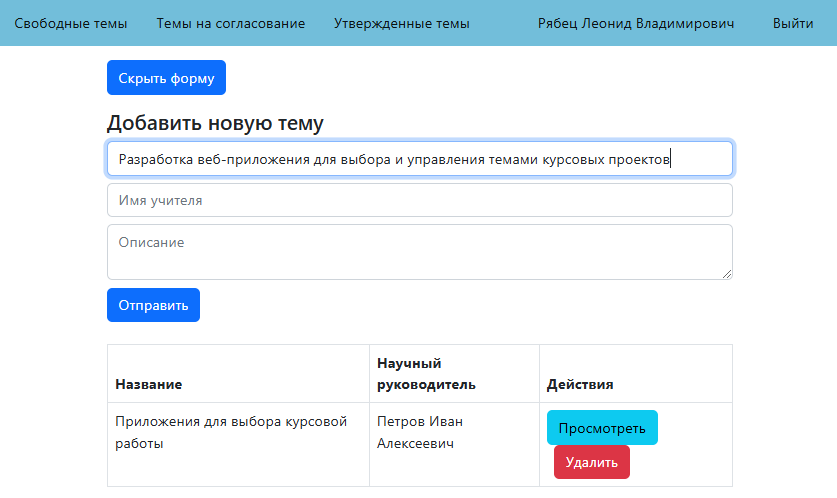
\includegraphics[width=0.8\textwidth]{cap1/nov.png}}
	\caption{Добавление новой темы}
	\label{ris1}
\end{figure}

Для студентов форма со всеми темами выглядит следующим образом. Для них отображается кнопка "выбрать" позволяющая выбрать себе данную тему курсовой работы

\begin{figure}[h]
	\centering	\fbox{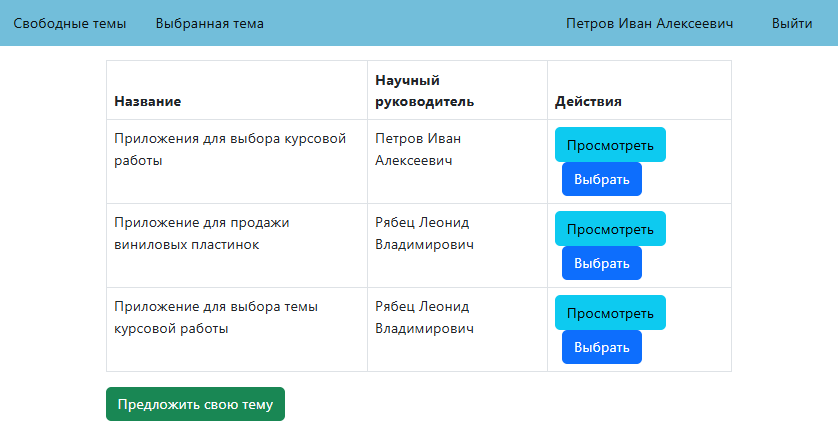
\includegraphics[width=0.8\textwidth]{cap1/stud.png}}
	\caption{Свободные темы}
	\label{ris1}
\end{figure}
\newpage
При нажатии на кнопку "Предолжить свою тему" \, или "Выбранная тема" \, студент попадет на страницу, если у студента выбрана тема, там будет отображаться выбранная тема, если он предлагал тему будет предложенная тема или форма для предложения темы.

\begin{figure}[h]
	\centering	\fbox{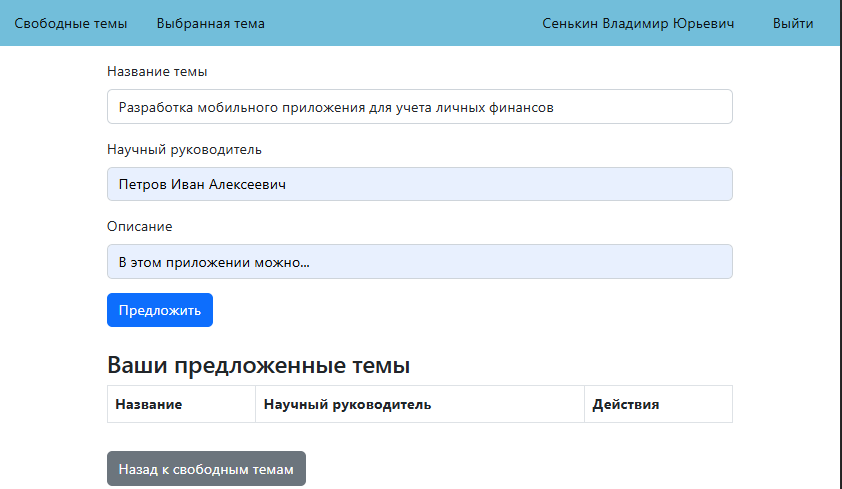
\includegraphics[width=0.8\textwidth]{cap1/stud2.png}}
	\caption{Предложить свою тему}
	\label{ris1}
\end{figure}

После добавления выбора темы студент может откзаться от темы, а также посмотреть комментарий преподавателя.

\begin{figure}[h]
	\centering	\fbox{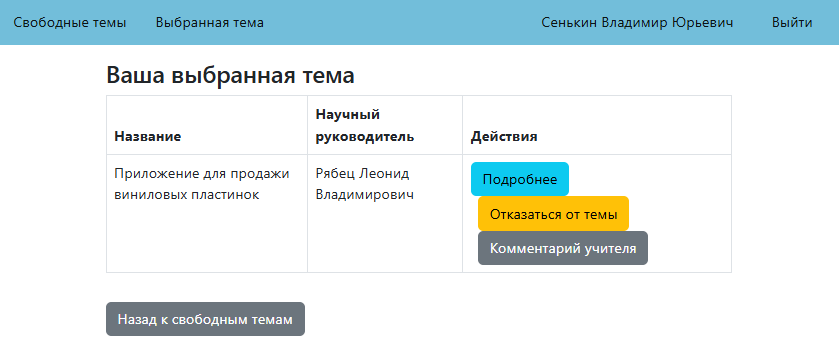
\includegraphics[width=0.8\textwidth]{cap1/stud3.png}}
	\caption{Ваша выбранная тема}
	\label{ris1}
\end{figure}

%-------------
%Заключение 
%-------------
\mynonumbersection{ЗАКЛЮЧЕНИЕ}

В результате проделанной работы было создано веб-приложение для выбора тем курсовых, которое удовлетворяет потребностям преподавателей и студентов.

Цели и задачи проекта были успешно достигнуты:
\begin{itemize}
\item Реализован компактный список свободных тем курсовых работ.
\item Реализована возможность комментирования тем курсовых работ.
\item Реализована различная функциональность дял разных пользователей.
\item Реализована регистрация и авторизация пользователей.
\item Реализована возможность предложения своей темы.
\end{itemize}

Планируется значительное расширение функциональности проекта в будущем, включая полную реализацию системы сообщений между студентами и преподавателями. Эти дополнения позволят студентам удобно взаимодействовать с преподователями и быстрее выбирать тподходящую темы.
    
%-------------
%Список литературы
%-------------
\newpage
%Для включения в диплом списка литературы подключается файл literature.bib
%В нем приведены наиболее часто встречающиеся типы библиографических ссылок
\renewcommand{\refname}{СПИСОК ИСПОЛЬЗОВАННЫХ ИСТОЧНИКОВ}
\addcontentsline{toc}{section}{\refname}
\printbibliography

%-------------
%Приложения
%-------------
\addappendix{Контроллер свободных тема}
\label{topicFreeController}

\begin{lstlisting}[language=Java, caption={Контроллер свободных тем}]
RestController
@RequestMapping("/api")
@CrossOrigin(origins = "*", maxAge = 3600)
public class TopicFreeController {

    @Autowired
    private TopicFreeRepository topicFreeRepository;

    @Autowired
    private TopicFreeService topicFreeService;

    @Autowired
    private TopicLockService topicLockService;

    @Autowired
    private UserService userService;

    @GetMapping("/topicfree")
    public ResponseEntity<List<TopicFree>> getAllFreeTopics() {
        List<TopicFree> topicfree = topicFreeRepository.findAll();
        return ResponseEntity.ok(topicfree);
    }
    // Добавление новой темы
    @PostMapping("/add")
    public ResponseEntity<TopicFree> addTopic(@RequestBody TopicFree newTopic) {
        TopicFree createdTopic = topicFreeService.addTopic(newTopic);
        return ResponseEntity.ok(createdTopic);
    }
    // Удаление темы
    @DeleteMapping("/delete/{topicId}")
    public ResponseEntity<Void> deleteTopic(@PathVariable Integer topicId) {
        topicFreeService.deleteTopic(topicId);
        return ResponseEntity.ok().build();
    }
    // Выбор темы
    @PostMapping("/select")
    public ResponseEntity<String> selectTopic(@RequestBody TopicSelectionRequest request){
        TopicFree selectedTopic = topicFreeService.getTopicById(request.getTopicId());
        if (topicLockService.isTopicSelectedByUser(request.getUserId())) {
            return new ResponseEntity<>("Вы уже выбрали тему!", HttpStatus.CONFLICT);
        }
        TopicLock topicLock = new TopicLock();
        topicLock.setName(selectedTopic.getName());
        topicLock.setTeacher(selectedTopic.getTeacher());
        topicLock.setDescription(selectedTopic.getDescription());
        topicLock.setUserId(request.getUserId());
        topicLock.setUsername(userService.getUsernameById(request.getUserId()));
        topicLockService.addTopicLock(topicLock);
        topicFreeService.deleteTopic(request.getTopicId());
        return new ResponseEntity<>("Тема успешно выбрана", HttpStatus.OK);}}
\end{lstlisting}

\addappendix{Контроллер предложенных тем}
\label{suggestTopicController}

\begin{lstlisting}[language=Java, caption={Контроллер предложенных тем}]
@RestController
@RequestMapping("/api") // Базовый путь для запросов
@CrossOrigin(origins = "*", maxAge = 3600)
public class SuggestTopicController {

    @Autowired
    private SuggestTopicRepository SuggesttopicRepository;

    @Autowired
    private TopicLockService topicLockService;

    @Autowired
    private TopicFreeService topicFreeService;

    @Autowired
    private SuggestTopicService suggestTopicService;

    @Autowired
    private UserService userService;

    //Получение всех предложенных тем
    @GetMapping("/suggested-topics")
    public List<SuggestTopic> getSuggestedTopics() {
        return SuggesttopicRepository.findAll();
    }
    // Предложение новой темы
    @PostMapping("/suggest-topic")
    public ResponseEntity<SuggestTopic> suggestTopic(@RequestBody SuggestTopic suggestTopic) {
        suggestTopic.setComment("Нет комментария.");
        suggestTopic.setUsername(userService.getUsernameById(suggestTopic.getUserId()));
        System.out.println("SASUN");
        SuggestTopic savedTopic = SuggesttopicRepository.save(suggestTopic);
        return ResponseEntity.ok(savedTopic);
    }
    @GetMapping("/selected-topic/{userId}")
    public ResponseEntity<TopicLock> getSelectedTopic(@PathVariable Integer userId) {
        TopicLock selectedTopic = topicLockService.getSelectedTopicByUserId(userId);
        if (selectedTopic != null) {
            return ResponseEntity.ok(selectedTopic);
        } else {
            return ResponseEntity.notFound().build();}}
    // Выбор темы
    @PostMapping("/reject-topic")
    public ResponseEntity<String> rejectTopic(@RequestBody Integer topicId) {
        TopicLock selectedTopic = topicLockService.getTopicById(topicId);
        TopicFree newTopicFree = new TopicFree();
        newTopicFree.setName(selectedTopic.getName());
        newTopicFree.setTeacher(selectedTopic.getTeacher());
        newTopicFree.setDescription(selectedTopic.getDescription());
        topicFreeService.addTopic(newTopicFree);
        topicLockService.deleteTopic(topicId);
        return new ResponseEntity<>("Тема успешно выбрана", HttpStatus.OK);}
    @PostMapping("/submit-comment/{topicId}")
    public ResponseEntity<String> submitComment(@PathVariable Integer topicId, @RequestBody String comment) {
        try {
            SuggestTopic updatedTopic = suggestTopicService.updateComment(topicId, comment);
            return ResponseEntity.ok("Комментарий успешно сохранен для темы: " + updatedTopic.getName());
        } catch (Exception e) {
            return ResponseEntity.status(404).body("Ошибка: " + e.getMessage()); }}
        // Одобрение темы
    @PostMapping("/approve-topic/{topicId}")
    public ResponseEntity<Void> approveTopic(@PathVariable Integer topicId) {
        try {
           suggestTopicService.approveAndCopyTopic(topicId);
            return ResponseEntity.ok().build();
        } catch (Exception e) {
            return ResponseEntity.status(500).build(); } }}
\end{lstlisting}

\addappendix{Контроллер занятых тем}
\label{topicLockController}

\begin{lstlisting}[language=Java, caption={Контроллер занятх тем}]
@RestController
@RequestMapping("/api")
@CrossOrigin(origins = "*", maxAge = 3600)
public class TopicLockController {

    @Autowired
    private TopicFreeRepository topicFreeRepository;

    @Autowired
    private TopicFreeService topicFreeService;

    @Autowired
    private TopicLockService topicLockService;

    @Autowired
    private UserRepository userRepository;

    @GetMapping("/approved-topics")
    public ResponseEntity<List<TopicLock>> getApprovedTopics() {
        List<TopicLock> approvedTopics = topicLockService.getAllApprovedTopics();
        return ResponseEntity.ok(approvedTopics);}

    @DeleteMapping("/delete-topic/{id}")
    public ResponseEntity<String> deleteTopic(@PathVariable Integer id) {
        boolean isDeleted = topicLockService.deleteTopicById(id);
        if (isDeleted) {
            return ResponseEntity.ok("Тема успешно удалена.");
        } else {
            return ResponseEntity.status(404).body("Тема не найдена.");}}
    @PostMapping("/make-free/{topicId}")
    public ResponseEntity<String> makeTopicFree(@PathVariable Integer topicId) {
        // Получаем тему из topiclock
        TopicLock topicLock = topicLockService.getTopicById(topicId);
        if (topicLock == null) {
            return ResponseEntity.status(HttpStatus.NOT_FOUND).body("Тема не найдена.");}
        // Создаем новую тему для topicfree
        TopicFree topicFree = new TopicFree();
        topicFree.setName(topicLock.getName());
        topicFree.setTeacher(topicLock.getTeacher());
        topicFree.setDescription(topicLock.getDescription());
        topicFreeService.saveTopic(topicFree);
        topicLockService.deleteTopic(topicId);
        return ResponseEntity.ok("Тема успешно сделана свободной."); }
    @GetMapping("/username")
    public ResponseEntity<String> getUsernameById(@PathVariable Integer id) {
        Optional<User> userOpt = userRepository.findById(id);
        System.out.println("KKAL");
        if (userOpt.isPresent()) {
            return ResponseEntity.ok(userOpt.get().getUsername());
        } else {
            return ResponseEntity.status(HttpStatus.NOT_FOUND).body("Пользователь не найден");} }}
\end{lstlisting}

\addappendix{Клиентская часть ApprovedTopicsList}
\label{approvedTopicsList}

\begin{lstlisting}[language=html, caption={Клиентская часть ApprovedTopicsList}]
const ApprovedTopicsList = ({ user }) => {
    const [topics, setTopics] = useState([]);
    const [loading, setLoading] = useState(true);
    const [error, setError] = useState(null);
    const [expandedTopic, setExpandedTopic] = useState(null);
    const [pendingDelete, setPendingDelete] = useState(null);
    const [pendingMakeFree, setPendingMakeFree] = useState(null); 
    const [usernames, setUsernames] = useState({});

    useEffect(() => {
        const fetchTopics = async () => {
            try {
                const response = await http.get("/approved-topics");
                setTopics(response.data);
            } catch (err) {
                setError("Не удалось загрузить темы.");
                console.error(err);
            } finally {
                setLoading(false);
            }
        };
        fetchTopics(); }, []);
     // Функция для получения username по userId
     const fetchUsername = async (userId) => {
        try {
            const response = await http.get(`/username`, userId);
            return response.data;
        } catch (error) {
            console.error("Ошибка при получении имени пользователя:", error);
            return "Неизвестный пользователь"; }};
    const handleDelete = async (topicId) => {
        if (pendingDelete === topicId) {
            try {
                await http.delete(`/delete-topic/${topicId}`);
                setTopics(topics.filter(topic => topic.id !== topicId));
                setPendingDelete(null);
            } catch (error) {
                console.error("Ошибка при удалении темы:", error);
            }
        } else {
            setPendingDelete(topicId); } };
    const handleMakeFree = async (topicId) => {
        if (pendingMakeFree === topicId) {
            try {
                await http.post(`/make-free/${topicId}`);
                setTopics(topics.filter(topic => topic.id !== topicId)); 
                setPendingMakeFree(null); 
            } catch (error) {
                console.error("Ошибка при изменении статуса темы:", error);
            }
        } else {
            setPendingMakeFree(topicId);}};
    const toggleDescription = (id) => {
        setExpandedTopic(expandedTopic === id ? null : id);};
    if (loading) {
        return <div>Загрузка...</div>;}
    if (error) {
        return <div>{error}</div>;}
    return (
        <div className="container-md mt-3">
            <h2>Утвержденные темы</h2>
            <table className="table table-bordered">
                <thead>
                    <tr>
                        <th>Имя студента</th>
                        <th>Название</th>
                        <th>Преподаватель</th>
                        <th>Действия</th>
                    </tr>
                </thead>
                <tbody>
                    {topics.map((topic) => (
                        <React.Fragment key={topic.id}>
                            <tr>
                                <td>{topic.username}</td> {}
                                <td>{topic.name}</td>
                                <td>{topic.teacher}</td>
                                <td>
                                    <button 
                                        className="btn btn-info" 
                                        onClick={() => toggleDescription(topic.id)}
                                    >
                                        Просмотреть
                                    </button>
                                    <button 
                                        className={`btn ${pendingDelete === topic.id ? 'btn-warning' : 'btn-danger'} ms-2`} 
                                        onClick={() => handleDelete(topic.id)}
                                    >
                                        {pendingDelete === topic.id ? 'Подтвердить удаление' : 'Удалить'}
                                    </button>
                                    {pendingMakeFree === topic.id ? (
                                        <button 
                                            className="btn btn-success ms-2"
                                            onClick={() => handleMakeFree(topic.id)}
                                        >
                                            Подтвердить
                                        </button>
                                    ) : (
                                        <button 
                                            className="btn btn-secondary ms-2" 
                                            onClick={() => handleMakeFree(topic.id)}
                                        >
                                            Сделать свободной
                                        </button>
                                    )}
                                </td>
                            </tr>
                            {expandedTopic === topic.id && (
                                <tr>
                                    <td colSpan="4">
                                        <div className="p-3 border rounded">
                                            <p>{topic.description || 'Описание отсутствует.'}</p>
                                        </div>
                                    </td>
                                </tr>
                            )}
                        </React.Fragment>
                    ))}
                </tbody>
            </table>
        </div>
    );
};

export default ApprovedTopicsList;
\end{lstlisting}

\addappendix{Клиентская часть SuggestTopic}
\label{suggestTopic}

\begin{lstlisting}[language=html, caption={Клиентская часть SuggestTopic}]
const SuggestTopic = ({ user }) => {
    const [topicName, setTopicName] = useState('');
    const [topicTeacher, setTopicTeacher] = useState('');
    const [topicDescription, setTopicDescription] = useState('');
    const [suggestedTopics, setSuggestedTopics] = useState([]);
    const [selectedTopic, setSelectedTopic] = useState(null);
    const [showDescription, setShowDescription] = useState(false);
    const [confirmReject, setConfirmReject] = useState(false);
    const [activeTopicId, setActiveTopicId] = useState(null); 

    const navigate = useNavigate();
    const currentUser = user;

    useEffect(() => {
        if (!currentUser) {
            navigate('/TopicFreeList');} }, [currentUser, navigate]);

    useEffect(() => {
        if (currentUser) {
            http.get("/suggested-topics")
                .then(response => {
                    const userTopics = response.data.filter(topic => topic.userId === currentUser.id);
                    setSuggestedTopics(userTopics);
                })
                .catch(e => {console.log(e);});
            http.get(`/selected-topic/${currentUser.id}`)
                .then(response => {
                    if (response.data) {
                        setSelectedTopic(response.data); }})
                .catch(e => {
                    console.log(e);
                });
        }
    }, [currentUser]);
    const handleSubmit = (e) => {
        e.preventDefault();
        const newTopic = {
            name: topicName,
            teacher: topicTeacher,
            description: topicDescription,
            userId: currentUser.id,
        };
        http.post("/suggest-topic", newTopic)
            .then(response => {
                console.log("Topic suggested:", response.data);
                setSuggestedTopics([...suggestedTopics, response.data]);
                setTopicName('');
                setTopicTeacher('');
                setTopicDescription('');})
            .catch(error => {
                console.error("Error while suggesting topic:", error);});};
    const handleApprove = (topicId) => {
        http.post(`/approve-topic/${topicId}`)
            .then(response => {
                console.log("Topic approved:", response.data);
                setSuggestedTopics(suggestedTopics.map(topic =>
                    topic.id === topicId ? { ...topic, approved: true } : topic
                ));
            })
            .catch(error => {
                console.error("Error while approving topic:", error);}); };

    const handleReject = () => {
        if (confirmReject) {
            if (selectedTopic) {
                http.post(`/reject-topic`, selectedTopic.id)
                    .then(() => {
                        setSelectedTopic(null);
                        console.log("Topic rejected.");
                    })
                    .catch(error => {
                        console.error("Error while rejecting topic:", error);}); }
        } else {
            setConfirmReject(true); } };
    const handleDelete = (topicId) => {
        http.delete(`/delete-topic/${topicId}`)
            .then(() => {
                setSuggestedTopics(suggestedTopics.filter(topic => topic.id !== topicId));
                console.log("Topic deleted."); })
            .catch(error => {
                console.error("Error while deleting topic:", error);});};

    const toggleDescription = () => {
        setShowDescription(!showDescription);
    };

    const toggleTeacherComment = (topicId) => {
        setActiveTopicId(activeTopicId === topicId ? null : topicId);
    };

    return (
        <div className="container-md mt-3">
            {selectedTopic ? (
                <>
                    <h3>Ваша выбранная тема</h3>
                    <table className="table table-bordered mt-2">
                        <thead>
                            <tr>
                                <th>Название</th>
                                <th>Научный руководитель</th>
                                <th>Действия</th>
                            </tr>
                        </thead>
                        <tbody>
                            <tr>
                                <td>{selectedTopic.name}</td>
                                <td>{selectedTopic.teacher}</td>
                                <td>
                                    <button onClick={toggleDescription} className="btn btn-info">
                                        {showDescription ? "Скрыть описание" : "Подробнее"}
                                    </button>
                                    <button onClick={handleReject} className={`btn ${confirmReject ? "btn-danger" : "btn-warning"} ms-2`}>
                                        {confirmReject ? "Подтвердить отказ" : "Отказаться от темы"}
                                    </button>
                                    <button onClick={() => toggleTeacherComment(selectedTopic.id)} className="btn btn-secondary ms-2">
                                        {activeTopicId === selectedTopic.id ? "Скрыть комментарий" : "Комментарий учителя"}
                                    </button>
                                </td>
                            </tr>
                        </tbody>
                    </table>
                    {showDescription && (
                        <div className="alert alert-info mt-3">
                            <strong>Описание:</strong> {selectedTopic.description}
                        </div>
                    )}
                    {activeTopicId === selectedTopic.id && (
                        <div className="alert alert-secondary mt-3">
                            <strong>Комментарий учителя:</strong> {selectedTopic.comment || 'Нет комментария'}
                        </div>
                    )}
                </>
            ) : (
                <>
                    <form onSubmit={handleSubmit}>
                        <div className="mb-3">
                            <label htmlFor="topicName" className="form-label">Название темы</label>
                            <input
                                type="text"
                                className="form-control"
                                id="topicName"
                                value={topicName}
                                onChange={(e) => setTopicName(e.target.value)}
                                required
                            />
                        </div>
                        <div className="mb-3">
                            <label htmlFor="topicTeacher" className="form-label">Научный руководитель</label>
                            <input
                                type="text"
                                className="form-control"
                                id="topicTeacher"
                                value={topicTeacher}
                                onChange={(e) => setTopicTeacher(e.target.value)}
                                required
                            />
                        </div>
                        <div className="mb-3">
                            <label htmlFor="topicDescription" className="form-label">Описание</label>
                            <input
                                type="text"
                                className="form-control"
                                id="topicDescription"
                                value={topicDescription}
                                onChange={(e) => setTopicDescription(e.target.value)}
                                required
                            />
                        </div>
                        <button type="submit" className="btn btn-primary">Предложить</button>
                    </form>
                </>
            )}

            {!selectedTopic && (
                <>
                    <h3 className="mt-4">Ваши предложенные темы</h3>
                    <table className="table table-bordered mt-2">
                        <thead>
                            <tr>
                                <th>Название</th>
                                <th>Научный руководитель</th>
                                <th>Действия</th>
                            </tr>
                        </thead>
                        <tbody>
                            {suggestedTopics.map((topic, i) => (
                                <tr key={i}>
                                    <td>{topic.name}</td>
                                    <td>{topic.teacher}</td>
                                    <td>
                                        <button onClick={() => toggleTeacherComment(topic.id)} className="btn btn-secondary ms-2">
                                            {activeTopicId === topic.id ? "Скрыть комментарий" : "Комментарий учителя"}
                                        </button>
                                        {currentUser?.role === "ROLE_ADMIN" && (
                                            <>
                                                <button onClick={() => handleApprove(topic.id)} className="btn btn-success ms-2">
                                                    Одобрить
                                                </button>
                                                <button onClick={() => handleDelete(topic.id)} className="btn btn-danger ms-2">
                                                    Удалить
                                                </button>
                                            </>
                                        )}
                                    </td>
                                </tr>
                            ))}
                        </tbody>
                    </table>
                    {activeTopicId && suggestedTopics.find(topic => topic.id === activeTopicId)?.comment && (
                        <div className="alert alert-secondary mt-3">
                            <strong>Комментарий учителя:</strong> {suggestedTopics.find(topic => topic.id === activeTopicId).comment}
                        </div>
                    )}
                </>
            )}

            {currentUser?.role === "ROLE_USER" && (
                <Link to="/TopicFreeList" className="btn btn-secondary mt-3">Назад к свободным темам</Link>
            )}
        </div>
    );
};
// Redux
function mapStateToProps(state) {
    const { user } = state.auth;
    return { user};}
export default connect(mapStateToProps)(SuggestTopic);
\end{lstlisting}

\addappendix{Клиентская часть TopicFreeList}
\label{topicFreeList}

\begin{lstlisting}[language=html, caption={Клиентская часть TopicFreeList}]
const TopicFreeList = ({ user }) => {
    const [topicfreeall, setCategories] = useState([]);
    const [expandedTopic, setExpandedTopic] = useState(null);
    const [selectedTopic, setSelectedTopic] = useState(null);
    const [newTopic, setNewTopic] = useState({
        name: '',
        teacher: '',
        description: ''});
    const [isFormVisible, setIsFormVisible] = useState(false);
    const [pendingDelete, setPendingDelete] = useState(null);
    useEffect(() => {
        http.get("/topicfree")
            .then(response => {
                setCategories(response.data);
            })
            .catch(e => {
                console.log(e); });}, []);
    const toggleDescription = (id) => {
        setExpandedTopic(expandedTopic === id ? null : id); };
    const handleSelectTopic = (topicId) => {
        if (selectedTopic === topicId) {
            setSelectedTopic(null); 
        } else {
            setSelectedTopic(topicId);  }};
    const handleConfirmTopic = () => {
        if (!selectedTopic) return;
        const requestBody = {
            topicId: selectedTopic,
            userId: user.id };
        http.post(`/select`, requestBody)
        .then((response) => {
            alert(response.data); 
            setCategories(topicfreeall.filter(t => t.id !== selectedTopic)); 
            setSelectedTopic(null);  })
        .catch((error) => {
            if (error.response && error.response.status === 409) {
                alert("Невозможно выбрать больше одной темы!"); 
            } else {
                console.error('Error selecting topic:', error);
                alert("Ошибка при выборе темы"); } });};
    const handleDeleteTopic = (topicId) => {
        if (pendingDelete === topicId) {
            http.delete(`/delete/${topicId}`)
                .then(() => {
                    setCategories(topicfreeall.filter(t => t.id !== topicId));
                    setPendingDelete(null);  })
                .catch((e) => {
                    console.error('Error deleting topic:', e); });
        } else {
            setPendingDelete(topicId);} };
    const handleAddTopic = () => {
        http.post("/add", newTopic)
            .then(response => {
                setCategories([...topicfreeall, response.data]);
                setNewTopic({ name: '', teacher: '', description: '' });
                setIsFormVisible(false); })
            .catch(e => {
                console.error('Error adding topic:', e);});};
    return (
        <div className="container-md mt-3">
            {user && user.role === 'ROLE_ADMIN' && (
                <div className="mb-4">
                    <button 
                        className="btn btn-primary" 
                        onClick={() => setIsFormVisible(!isFormVisible)}>
                        {isFormVisible ? 'Скрыть форму' : 'Добавить новую тему'}
                    </button>
                    {isFormVisible && (
                        <div className="mt-3">
                            <h4>Добавить новую тему</h4>
                            <div className="mb-2">
                                <input 
                                    type="text" 
                                    placeholder="Название темы" 
                                    value={newTopic.name} 
                                    onChange={(e) => setNewTopic({ ...newTopic, name: e.target.value })} 
                                    className="form-control" 
                                />
                            </div>
                            <div className="mb-2">
                                <input 
                                    type="text" 
                                    placeholder="Имя учителя" 
                                    value={newTopic.teacher} 
                                    onChange={(e) => setNewTopic({ ...newTopic, teacher: e.target.value })} 
                                    className="form-control" 
                                />
                            </div>
                            <div className="mb-2">
                                <textarea 
                                    placeholder="Описание" 
                                    value={newTopic.description} 
                                    onChange={(e) => setNewTopic({ ...newTopic, description: e.target.value })} 
                                    className="form-control" 
                                />
                            </div>
                            <button 
                                className="btn btn-primary" 
                                onClick={handleAddTopic}
                            >
                                Отправить
                            </button>
                        </div>
                    )}
                </div>
            )}
            <div className="col-sm-12 mt-2">
                <table className="table table-bordered">
                    <thead>
                        <tr>
                            <th>Название</th>
                            <th>Научный руководитель</th>
                            <th>Действия</th>
                        </tr>
                    </thead>
                    <tbody>
                        {topicfreeall.map((topicfree, i) => (
                            <React.Fragment key={i}>
                                <tr>
                                    <td>{topicfree.name}</td>
                                    <td>{topicfree.teacher}</td>
                                    <td>
                                        {}
                                        <button 
                                            className="btn btn-info" 
                                            onClick={() => toggleDescription(topicfree.id)}
                                        >
                                            Просмотреть
                                        </button>
                                        {user && user.role === 'ROLE_USER' && (
                                            <>
                                                <button 
                                                    className="btn btn-primary ms-2"
                                                    onClick={() => handleSelectTopic(topicfree.id)}
                                                >
                                                    {selectedTopic === topicfree.id ? 'Выбрана' : 'Выбрать'}
                                                </button>

                                                {}
                                                {selectedTopic === topicfree.id && (
                                                    <button 
                                                        className="btn btn-success ms-2"
                                                        onClick={handleConfirmTopic}
                                                    >
                                                        Подтвердить
                                                    </button>
                                                )}
                                            </>
                                        )}
                                        {user && user.role === 'ROLE_ADMIN' && (
                                            <button 
                                                className={`btn ${pendingDelete === topicfree.id ? 'btn-warning' : 'btn-danger'} ms-2`} 
                                                onClick={() => handleDeleteTopic(topicfree.id)}
                                            >
                                                {pendingDelete === topicfree.id ? 'Подтвердить удаление' : 'Удалить'}
                                            </button>
                                        )}
                                    </td>
                                </tr>
                                {expandedTopic === topicfree.id && (
                                    <tr>
                                        <td colSpan="3">
                                            <div className="p-3 border rounded">
                                                <p>{topicfree.description || 'Описание отсутствует.'}</p>
                                            </div>
                                        </td>
                                    </tr>
                                )}
                            </React.Fragment>
                        ))}
                    </tbody>
                </table>
            </div>
            {user && user.role === 'ROLE_USER' && (
                <div className="row">
                    <div className="col">
                        <Link to="/SuggestTopic" className="btn btn-success mb-3">Предложить свою тему</Link>
                    </div>
                </div> )}
        </div> );};
// Redux
function mapStateToProps(state) {
    const { user } = state.auth;
    return {user};}
export default connect(mapStateToProps)(TopicFreeList);
\end{lstlisting}


\end{document}

